
\section{Transferring models to Python}

\begin{figure}[h]
    \centering
    \addtolength{\leftskip} {-4cm}
    \addtolength{\rightskip}{-4cm}
    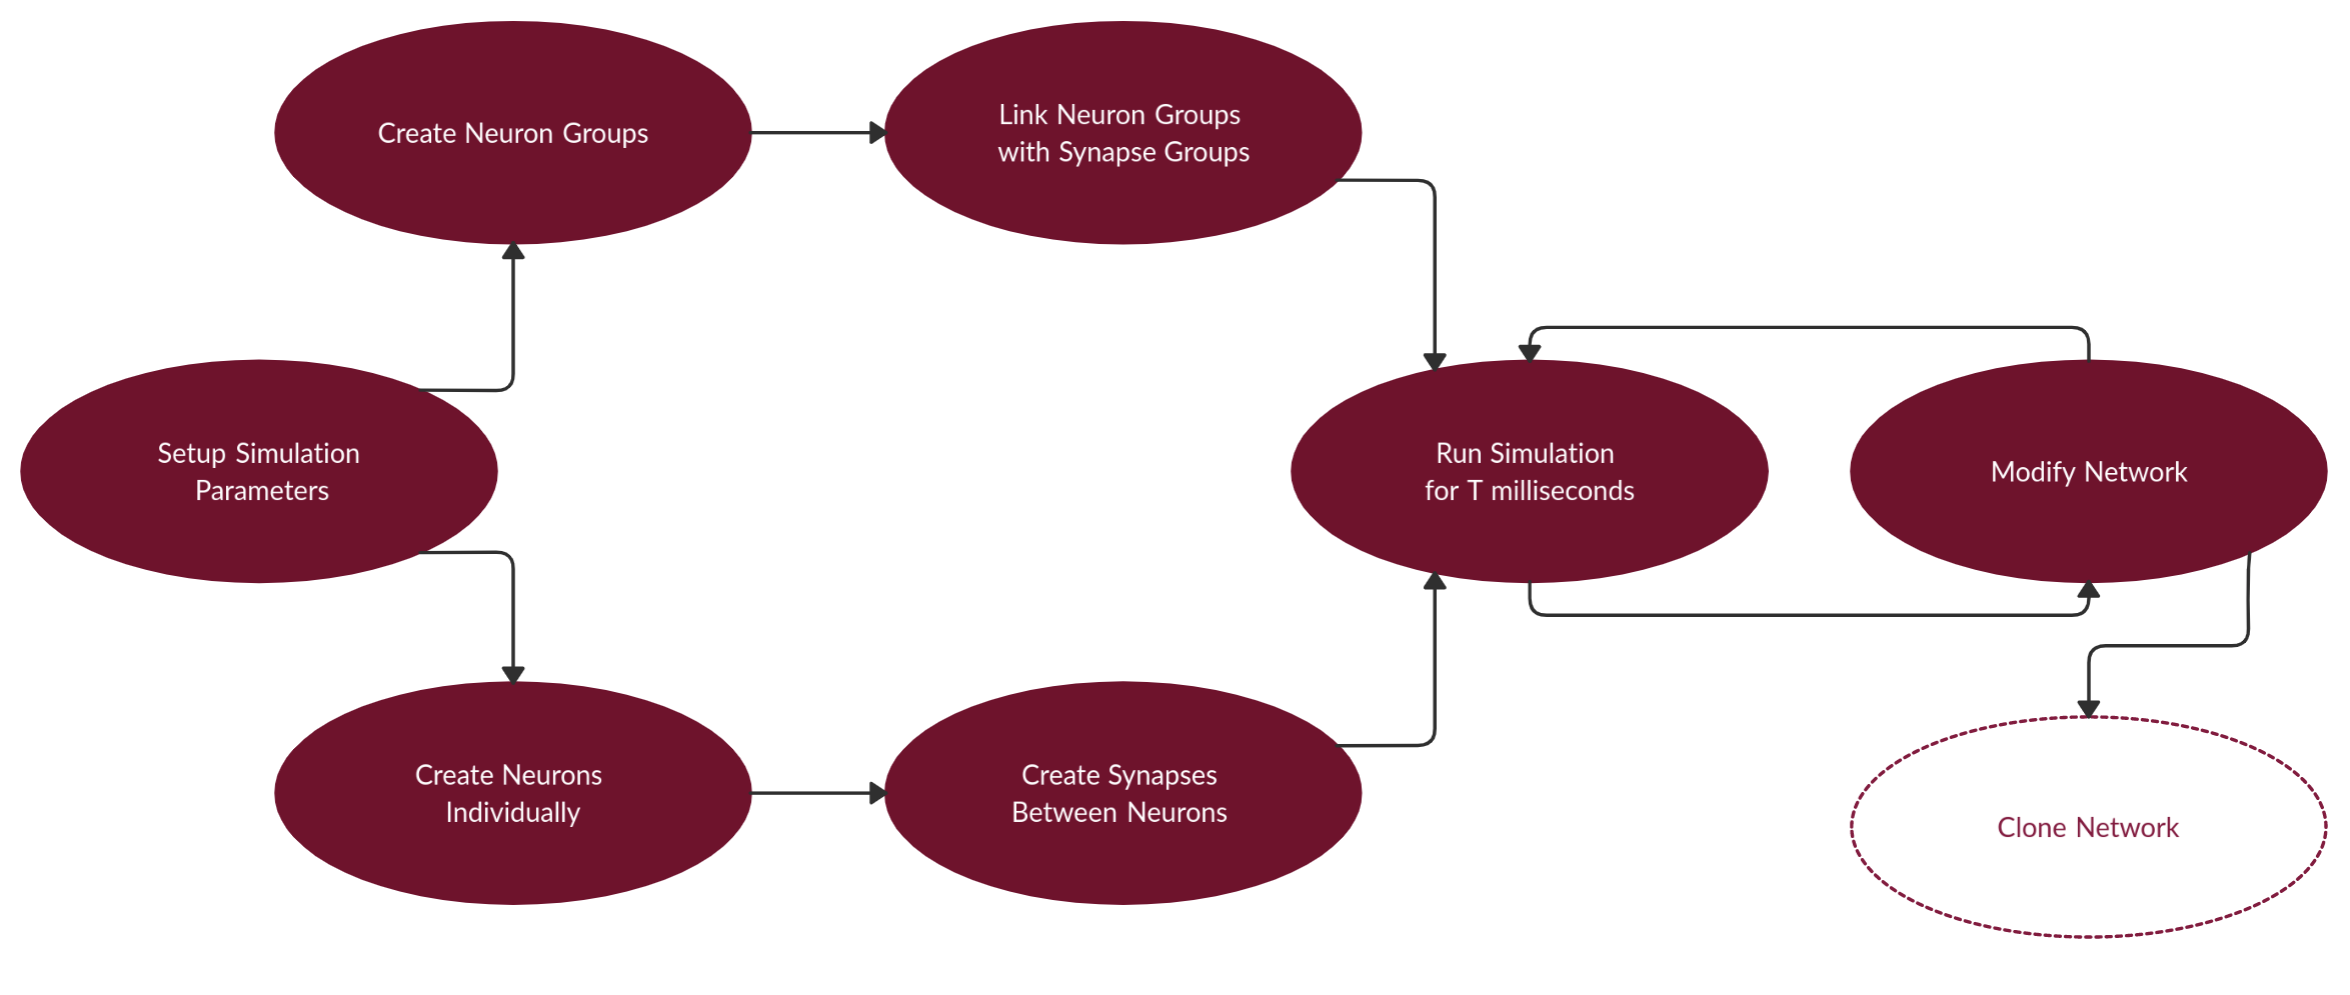
\includegraphics[width=1.3\linewidth]{figures/images/workflow.png}
    \caption{The simulation workflow}
    \label{fig:workflow}
\end{figure}

In order to flexibly mix object oriented and functional programming paradigms,
I've chosen to develop these models in the Python programming language. Python
is home to a healthy and active ecosystem of libraries and development practices
for scientific and statistical research to draw from. Of particular note are the
SciPy libraries, which provide a performant set of functions and objects that
speed up floating point arithmetic and vector mathematics. 

In figure \ref{fig:workflow}, the planned workflow for using the simulation is
mapped out, where the user can easily mix and match large probabilistically
generated networks and manually configured groups of neurons. It is in the
simulate and modify loop that experimentation can take place.

\subsection{Object oriented neurons}

In order to make the simulation as extensible as possible, I have chosen to
implement it in an object oriented manner, where functionality of the components
in a the neural network is compartmentalised to the objects that should own said
functionality. For instance, each neuron holds its state, and state history, and
the functions that modify that state.

Another significant advantage of using object oriented programming in Python is
that objects can be deeply cloned using Python's \texttt{copy} library, a significant benefit when it comes to
duplicating networks. 

\begin{figure}[h!]
    \centering
    % \addtolength{\leftskip} {-4cm}
    % \addtolength{\rightskip}{-4cm}
    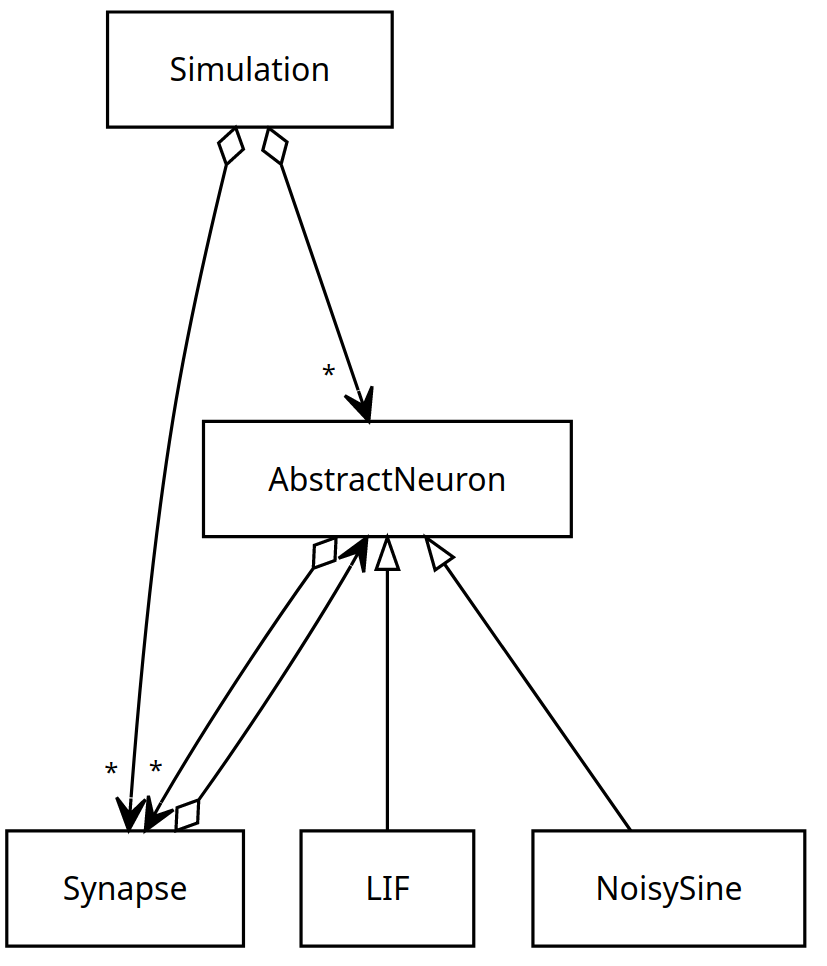
\includegraphics[width=0.5\linewidth]{figures/images/UML2.png}
    \caption{UML Diagram}
    \label{fig:uml}
\end{figure}

On a basic level, the hierarchy within the simulation is as follows: All neurons
and synapses belong to a Simulation object, and the neurons in the network are
doubly-linked with synapses in-between. This is illustrated in figure
\ref{fig:uml}. Neurons have been split into a base class \texttt{AbstractNeuron}
that holds the vector of input synapses and presents an interface to get the
neuron potential, but the specific implementation details are left to
\texttt{AbstractNeuron}'s implementations. One of these implementations is the
LIF neuron described earlier in this chapter, and the other is
\texttt{NoisySine}, a Neuron that uses overlapping sine-waves to generate an
output current. 

\subsection{Network Topology}

In order to model the passing of information through the simulation, there were
several approaches that I could take. In order to pick a solution, it is
necessary to map out the relationships between neurons in some sample topologies
and the features that need to be supported by the synapses in such topologies.

\subsubsection{Stochastic generation of networks}

When creating large networks of neurons, it is simpler to organise them in
groups that are generated with random variables, and to stochastically link
neuron groups with synapse groups. 

\subsubsection{Function parameters instead of static parameters}

It is desirable to make the parameters that define the random distribution in a group
generation function be configurable at runtime, but increasing the number of
parameters in a function signature increases the mental overhead when a programmer is
using an API [CITE THIS]. 

However,
this can be simplified even further by passing a single PYTHON CALLABLE, which
in practice is a closure that encapsulates a function that produces a
distribution of the user's choice. 